\section{Results}
\label{sec:results}

All accuracy numbers are reported on the held-out test split ($N = 2500$ scenarios) and, unless noted, in physical surface-elevation units obtained by reversing the target normalization. Following Section~\ref{subsec:eval-metrics}, the relative $L_2$ and maximum errors are accumulated globally over the whole split rather than averaged per batch. The FNO is trained and evaluated separately against each of the three numerical references; the expanded hydrostatic comparison set includes FFNO, mode-count ablations, U-FNO, WNO, U-Net, and CNN models.

\subsection{Reference-solver validation and dataset quality}
\label{subsec:res-dataset}

Each numerical reference is generated on the same scenario design, giving three parallel datasets (hydrostatic, MUSCL-HR, Boussinesq) of $13{,}500$ scenarios each, split into $10{,}000$ train, $1{,}000$ validation, and $2{,}500$ test rollouts with fixed, disjoint seeds. Every stored rollout is a $50$-frame $\eta$ trajectory on a $64\times64$ grid with the $C=3$ input stack of Section~\ref{subsec:forward-task}. Under the quality policy of Section~\ref{subsec:reference-validation}, all $13{,}500$ scenarios in each dataset pass with \texttt{quality\_status}~$=$~\texttt{ok}: no rollout is dropped for non-finite values, sub-tolerance depth, or amplitude violations, and for the Boussinesq reference the conjugate-gradient acceleration solve converged on every sample. The source-strength multiplier spans the same $[0.45,\, 0.85]$ range across all three solvers, and the six source families and five bathymetry types appear in matched proportions across the three references and across the train/validation/test splits, so a surrogate trained on one reference and a comparison against another see the same scenario population. Because the references share scenario IDs, the cross-solver gaps of Section~\ref{subsec:res-solver-fidelity} are computed on all $2{,}500$ shared test scenarios for each pair.

Table~\ref{tab:solver-validation} summarizes the final solver-validation pass used to justify the labels as clean numerical references. All three solvers preserve lake-at-rest to roundoff on the 24-sample randomized checks, all stored dynamic rollouts are finite across the $13{,}500$ samples per solver, and the Boussinesq acceleration solve has zero recorded conjugate-gradient failures. With sponge disabled for the conservation diagnostic, the shallow-water references keep the mass/free-surface integral to about $2.6 \times 10 ^ {-16}$. The CFL rows are included only as a timestep-sensitivity diagnostic at matched physical end time: CFL $0.60$ remains finite on the small subset but shows large final-field differences, so these numbers are not a convergence proof.

\begin{table}[!htbp]
\centering
\caption{Reference-solver validation summary. Lake-at-rest and conservation checks are rerun diagnostics on denormalized inputs; dynamic finite-state statistics are aggregated over the generated datasets. CFL sensitivity is diagnostic only.}
\label{tab:solver-validation}
\begin{tabular}{p{0.34\linewidth}p{0.25\linewidth}cc}
    \toprule
    Check & Solver & Samples & Result \\
    \midrule
    Lake at rest max $\eta$ drift           & Hydrostatic & $24$ & $8.88 \times 10 ^ {-16}$ \\
    Late at rest max $\eta$ drift           & MUSCL-HR    & $24$ & $5.33 \times 10 ^ {-15}$ \\
    Lake at rest max $\eta$ drift           & Boussinesq  & $24$ & $0$ \\
    Dynamic finite pass rate                & Hydrostatic / MUSCL-HR / Boussinesq & $13{,}500$ each & $1.000$ \\
    Boussinesq CG failures / max iterations & Boussinesq  & $13{,}500$ & $0$ / $416$ \\
    Max mass rel.\ change                   & Hydrostatic / MUSCL-HR & $24$ each & $\approx 2.6 \times 10 ^ {-16}$ \\
    CFL final-field sensitivity vs $0.45$   & Hydrostatic / MUSCL-HR & $12$ each & diagnostic \\
    \bottomrule
\end{tabular}
\end{table}

\subsection{Same-solver surrogate accuracy}
\label{subsec:res-accuracy}

Table~\ref{tab:accuracy} reports field accuracy for the direct single-pass models on the hydrostatic reference, together with the FNO trained against each of the three references. Against the hydrostatic reference the FFNO is the strongest direct model, reaching a relative $L_2$ of $0.168$ while using $0.411$M parameters, compared with $0.235$ and $5.443$M parameters for the base FNO (about $13 \times$ fewer). The base FNO, U-FNO, and FNO-modes20 are effectively tied around $0.235$, the lower-mode FNO-modes8 is slightly worse at $0.241$, and the WNO, U-Net, and plain CNN trail at $0.367$, $0.475$, and $0.607$. The ordering supports the need for global operator structure in this benchmark, but the small gap between several Fourier-family variants suggests that the main gain is not simply from increasing the retained Fourier modes.

\begin{table}[H]
\centering
\caption{Same-solver field accuracy on the held-out test split ($N = 2500$). Parameter counts are in millions. MAE and RMSE are in physical surface-elevation units; relative $L_2$ is dimensionless; max-err is the global worst-case element in normalized units. The first block shares the hydrostatic reference; the last two rows are the FNO trained and scored against the MUSCL-HR and Boussinesq references on their own test splits.}
\label{tab:accuracy}
\begin{tabular}{llccccc}
    \toprule
    Model & Reference & Params (M) & MAE & RMSE & rel-$L_2$ & max-err \\
    \midrule
    FFNO        & Hydrostatic & $0.411$  & $0.00066$ & $0.00163$ & $\mathbf{0.168}$ & $18.6$ \\
    FNO         & Hydrostatic & $5.443$  & $0.00087$ & $0.00227$ & $0.235$          & $22.9$ \\
    U-FNO       & Hydrostatic & $6.938$  & $0.00086$ & $0.00227$ & $0.235$          & $26.3$ \\
    FNO-modes20 & Hydrostatic & $11.083$ & $0.00088$ & $0.00228$ & $0.235$          & $24.4$ \\
    FNO-modes8  & Hydrostatic & $1.793$  & $0.00084$ & $0.00233$ & $0.241$          & $25.5$ \\
    WNO         & Hydrostatic & $2.016$  & $0.00151$ & $0.00355$ & $0.367$          & $23.3$ \\
    U-Net       & Hydrostatic & $0.104$  & $0.00187$ & $0.00460$ & $0.475$          & $27.4$ \\
    CNN         & Hydrostatic & $0.045$  & $0.00236$ & $0.00588$ & $0.607$          & $29.8$ \\
    \midrule
    FNO         & MUSCL-HR    & $5.443$  & $0.00119$ & $0.00281$ & $0.263$          & $22.1$ \\
    FNO         & Boussinesq  & $5.443$  & $0.00137$ & $0.00468$ & $0.210$          & $15.9$ \\
    \bottomrule
\end{tabular}
\end{table}

The FNO behaves consistently across the three references, with relative $L_2$ between $0.21$ and $0.26$. On the dimensionless relative $L_2$ it scores lowest on the Boussinesq target ($0.210$). This ranking is unit-dependent and should be read with care: in physical surface-elevation units the Boussinesq surrogate is actually the \emph{least} accurate of the three FNO same-solver runs (RMSE $0.00468$ vs $0.00227$ hydrostatic and $0.00281$ MUSCL-HR), and likewise has the largest physical maximum error. The dimensionless and normalized-unit metrics flatter Boussinesq because its target normalization scale is about $2.3 \times$ larger ($0.0221$ vs $0.0097$), which shrinks every error expressed relative to that scale. We therefore avoid calling any single reference ``best'' outright: the FNO emulates all three to a comparable dimensionless fidelity, and the physical-unit ranking favors the shallow-water targets. These are same-solver numbers, each surrogate scored against the reference it was trained on, so they measure emulation quality and are kept separate from the raw solver-vs-solver gaps in Section~\ref{subsec:res-solver-fidelity}.

\begin{figure}[H]
\centering
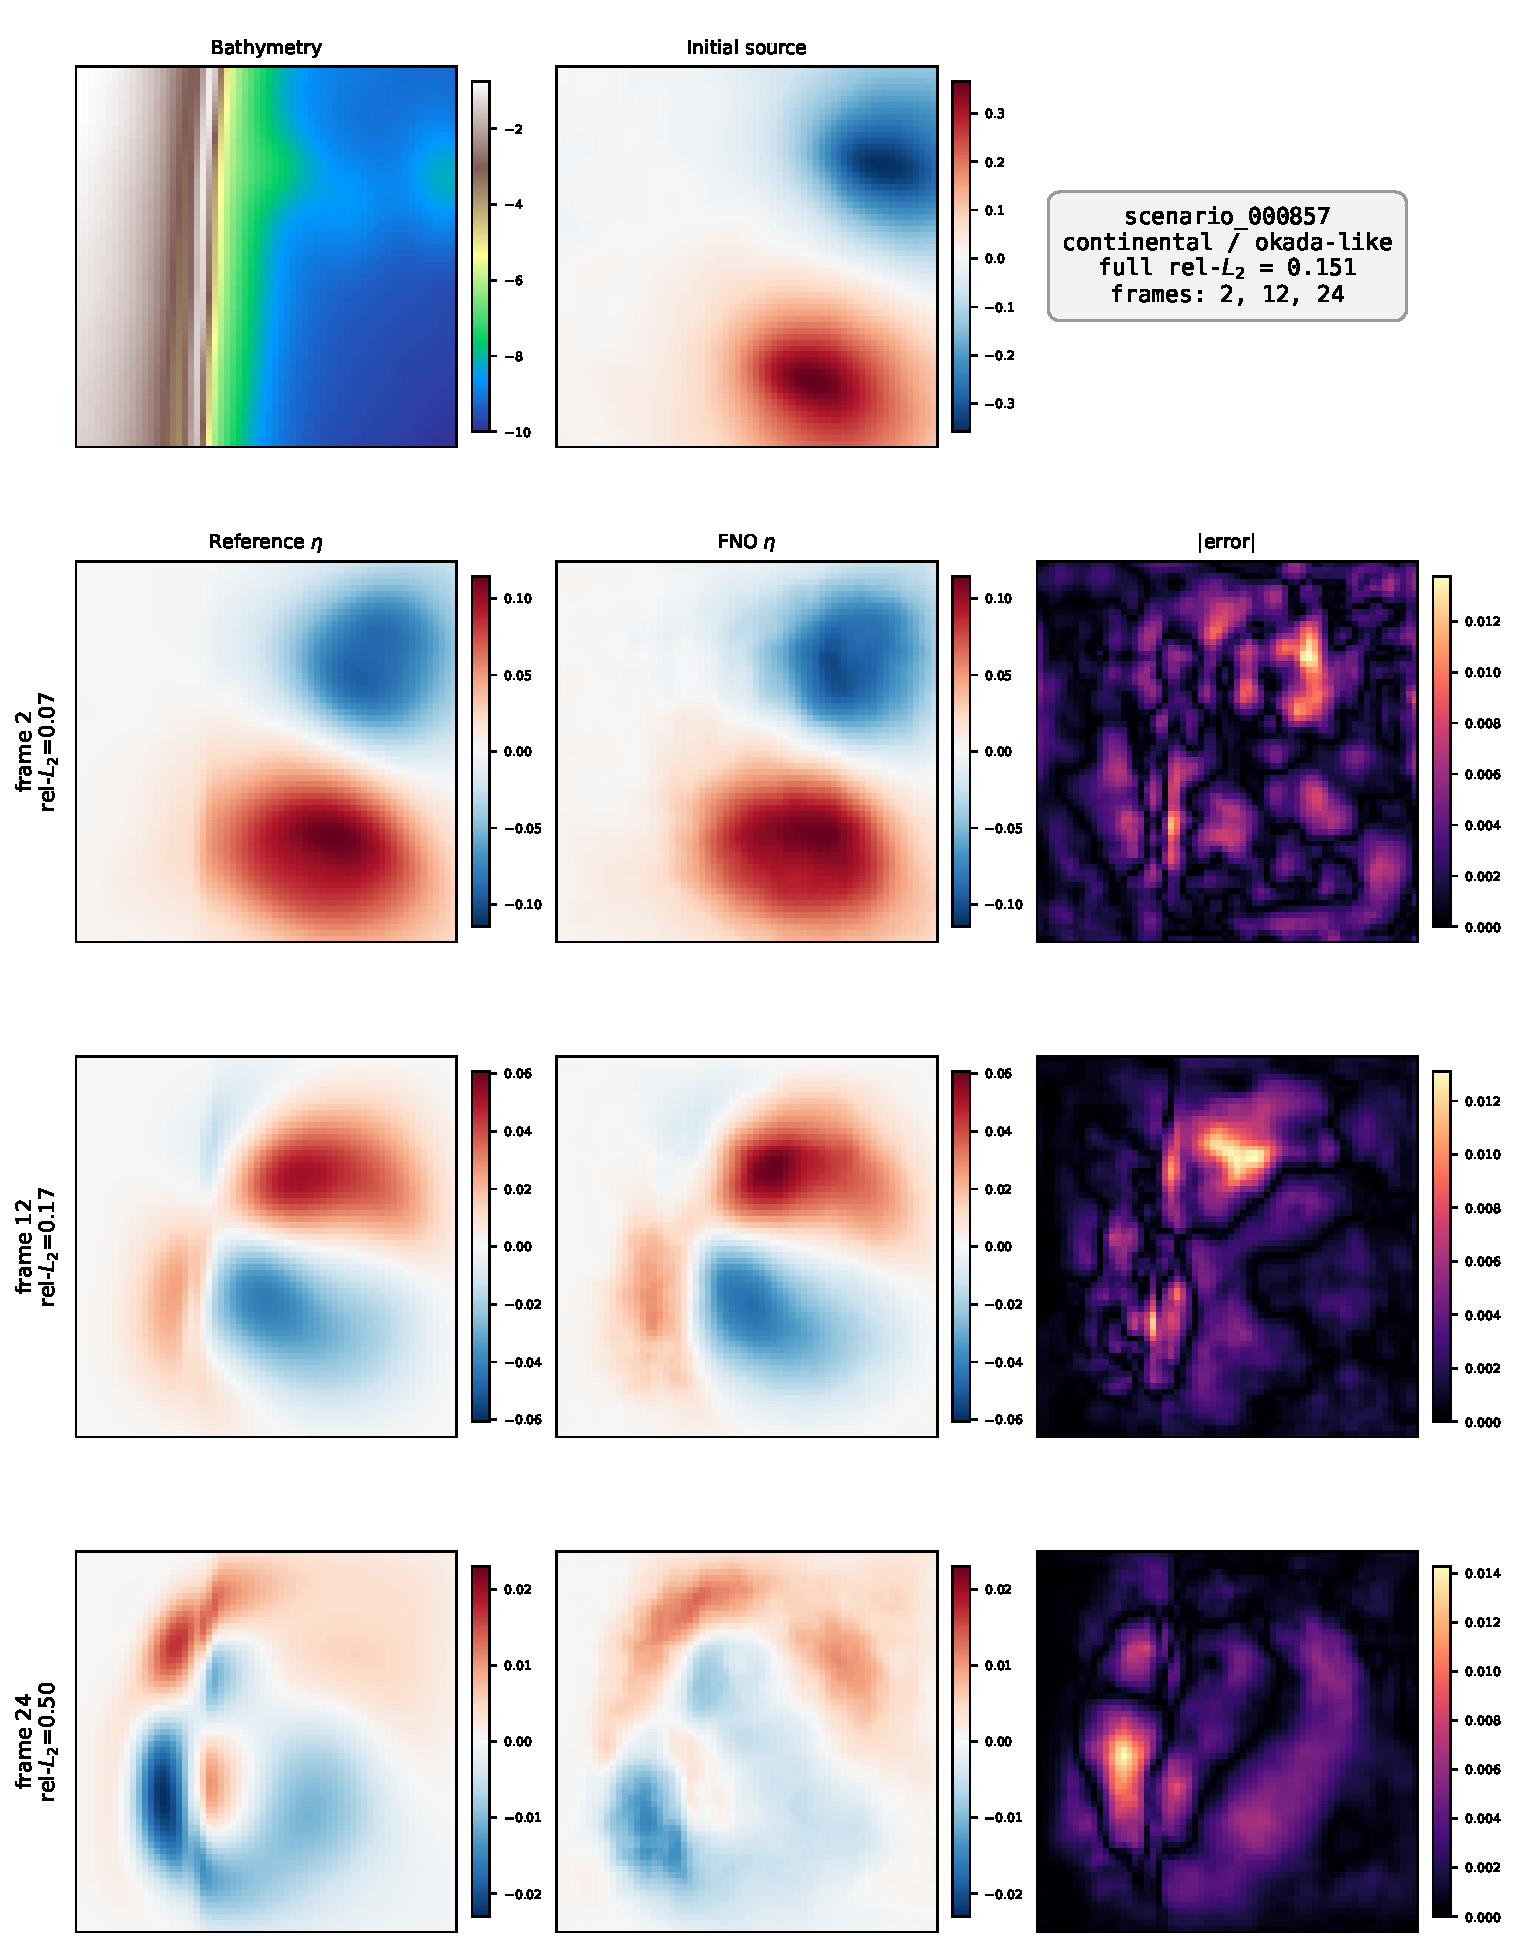
\includegraphics[width=0.9\linewidth]{figures/hydrostatic_rollout.pdf}
\caption{Qualitative single-pass FNO rollout on one hydrostatic test scenario (continental shelf--slope bathymetry with an Okada-like source). The top row shows the de-normalized bathymetry, the initial source, and the scenario metadata. Each lower row is one rollout frame (early, mid, late), showing the reference free surface $\eta$, the FNO prediction, and the absolute error in physical surface-elevation units. Within each frame row, the reference and prediction share the same symmetric $\eta$ scale, because the wavefield amplitude decays strongly over the horizon as the disturbance radiates out and the sponge layer damps it; the per-frame rel-$L_2$ rises accordingly, consistent with the trend in Table~\ref{tab:perframe}.}
\label{fig:rollout}
\end{figure}

\paragraph{Per-frame error growth.}
The single-pass models predict all $50$ frames in one shot, but their accuracy is not uniform over the forecast horizon, as the qualitative rollout in Figure~\ref{fig:rollout} already suggests. Table~\ref{tab:perframe} reports the per-frame relative $L_2$ at the first, middle, and last frame for the FNO on each reference and for the stronger hydrostatic FFNO. On the hydrostatic target the FNO error rises over the horizon, from $0.214$ at the first frame to a peak of $0.355$ late in the rollout (around frame $38$), then eases slightly to $0.309$ at the final frame, so the last frame is somewhat below the mid-to-late peak rather than the maximum. The FFNO lowers the whole curve, from $0.135$ at the first frame to $0.273$ at the last, but its peak still rises to $0.289$, so factorization reduces rather than removes drift. On MUSCL-HR the FNO error grows more steeply and does not recover, from $0.217$ to $0.469$ at the last frame -- the worst late-horizon drift of the three. This is the honest weakness of a horizon-predicting surrogate: even without an explicit autoregressive feedback loop, late frames depend on longer-range propagation and accumulate more error, the same drift pattern a recurrent rollout would show. The Boussinesq FNO is the clear exception: its per-frame error is essentially flat, $0.207$ at the first frame and $0.208$ at the last (range $0.205$--$0.217$), showing no temporal drift over the horizon. We attribute this to the smoothness of the weakly dispersive elevation field discussed above rather than to a different model, and we return to the drift-targeting windowed forecaster in Section~\ref{subsec:res-window}.

\begin{table}[!htbp]
\centering
\caption{Per-frame relative $L_2$ at the first frame, the mid-horizon frame, and the last frame of the $50$-step rollout ($N = 2500$). Numbers are in normalized units. FFNO reduces hydrostatic drift but does not remove it; the Boussinesq FNO remains nearly flat.}
\label{tab:perframe}
\begin{tabular}{llccc}
    \toprule
    Model & Reference & Frame $1$ & mid-horizon & frame $50$ \\
    \midrule
    FFNO & Hydrostatic & $0.135$ & $0.264$ & $0.273$ \\
    FNO  & Hydrostatic & $0.214$ & $0.325$ & $0.309$ \\
    FNO  & MUSCL-HR    & $0.217$ & $0.385$ & $0.469$ \\
    FNO  & Boussinesq  & $0.207$ & $0.206$ & $0.208$ \\
    \bottomrule
\end{tabular}
\end{table}

\paragraph{Physics diagnostics.}
Table~\ref{tab:physics-diag} gives three compact physics-aware diagnostics for the hydrostatic FNO and FFNO. The free-surface integral error measures the spatial-mean $\eta$ time series, the mass proxy uses the fully wet relation $h = \eta - b$, and the spectral-band rows split trajectory error by Fourier radius. These diagnostics track where the surrogate errors live; they do not imply that either network enforces conservation. The FFNO improves all three summaries, lowering the free-surface integral relative $L_2$ from $0.190$ to $0.139$ and the mass-proxy error from $1.20 \times 10 ^ {-4}$ to $8.77 \times 10 ^ {-5}$, while both models remain weakest in the high-wavenumber band.

\begin{table}[!htbp]
\centering
\caption{Hydrostatic physics diagnostics for direct single-pass FNO and FFNO on the held-out test split. Integral diagnostics are relative $L_2$ of spatial-mean time series; spectral columns are relative $L_2$ by Fourier band.}
\label{tab:physics-diag}
\begin{tabular}{lccccc}
    \toprule
    Model & $\eta$ integral & mass proxy & spectral low & spectral mid & spectral high \\
    \midrule
    FNO  & $0.190$ & $1.20 \times 10 ^ {-4}$ & $0.220$ & $0.499$ & $0.687$ \\
    FFNO & $0.139$ & $8.77 \times 10 ^ {-5}$ & $0.155$ & $0.452$ & $0.645$ \\
    \bottomrule
\end{tabular}
\end{table}

\subsection{Runtime and speedup}
\label{subsec:res-speed}

Table~\ref{tab:speed} reports per-sample timings from a dedicated benchmarking pass, following the protocol of Section~\ref{subsec:runtime}: GPU inference time per sample for each surrogate (CUDA, fp32), CPU rollout time per sample for each reference solver (rollout only, excluding bathymetry and source generation; float64), and their ratio as the speedup. The direct surrogates infer a full $50$-frame trajectory in roughly $0.17$~ms (CNN) to $3.89$~ms (U-FNO), against CPU solver rollouts of $16$--$72$~s per sample. The resulting speedups are large, from about $8.5 \times 10 ^ {3}$ for U-FNO against the hydrostatic solver up to about $1.9 \times 10 ^ {5}$ for the CNN against the same solver.

These ratios should be read as an order-of-magnitude, implementation-level comparison, not as a claim against optimized production tsunami codes. As stressed in Section~\ref{subsec:runtime}, the reference solvers are single-threaded CPU NumPy implementations chosen to be reproducible and auditable, not tuned for speed; a vectorized, compiled, or GPU solver would shrink the denominator substantially. The point is that even against an unoptimized baseline, the surrogate moves a per-scenario forecast from tens of seconds to milliseconds or less, which is the regime change that makes large ensemble or many-scenario studies practical. Among the FNO same-solver rows the speedup also tracks the cost of the target solver: the base FNO is fastest relative to MUSCL-HR ($\approx 7.99 \times 10 ^ {4}$), whose rollout is the most expensive ($72.34$~s), and slowest relative to Boussinesq ($\approx 1.82 \times 10 ^ {4}$), whose rollout is the cheapest ($16.48$~s).

\begin{table}[!htbp]
\centering
\caption{Per-sample runtime and speedup. Surrogate inference is timed on GPU (CUDA, fp32) over the full test split; reference-solver rollout is timed on CPU (float64) over $8$ scenarios with $3$ repeats, excluding bathymetry/source generation. Speedup is the solver rollout time per sample divided by the surrogate inference time per sample. These are implementation-level comparisons against unoptimized CPU reference solvers, not against optimized or GPU solvers (Section~\ref{subsec:runtime}).}
\label{tab:speed}
\begin{tabular}{lccrr}
    \toprule
    Model & Reference solver & Infer (ms) & Solver (s) & Speedup \\
    \midrule
    FNO         & Hydrostatic & $0.904$ & $33.06$ & $36{,}564  \times$ \\
    FFNO        & Hydrostatic & $1.664$ & $33.06$ & $19{,}873  \times$ \\
    CNN         & Hydrostatic & $0.171$ & $33.06$ & $192{,}921 \times$ \\
    U-Net       & Hydrostatic & $0.237$ & $33.06$ & $139{,}502 \times$ \\
    FNO-modes8  & Hydrostatic & $0.861$ & $33.06$ & $38{,}414  \times$ \\
    FNO-modes20 & Hydrostatic & $0.954$ & $33.06$ & $34{,}649  \times$ \\
    U-FNO       & Hydrostatic & $3.895$ & $33.06$ & $8{,}490   \times$ \\
    WNO         & Hydrostatic & $2.086$ & $33.06$ & $15{,}849  \times$ \\
    FNO         & MUSCL-HR    & $0.905$ & $72.34$ & $79{,}933  \times$ \\
    FNO         & Boussinesq  & $0.906$ & $16.48$ & $18{,}197  \times$ \\
    \bottomrule
\end{tabular}
\end{table}

\subsection{Distribution-shift generalization}
\label{subsec:res-ood}

Table~\ref{tab:ood} reports the hydrostatic FNO scored on the test pool grouped by source family. Following Section~\ref{subsec:generalization-protocol}, these are per-sample-then-grouped metrics, so the relative $L_2$ of a group is the mean of the per-sample values and is not directly comparable cell-for-cell with the globally aggregated number in Table~\ref{tab:accuracy}. All six families are present in the training distribution, so this is a difficult-subgroup analysis rather than a held-out-family test.

\begin{table}[!htbp]
\centering
\caption{Source-family breakdown for the hydrostatic FNO (per-sample-then-grouped, Section~\ref{subsec:generalization-protocol}). MAE is physical; rel-$L_2$ and max-err are per-sample means within the group; $n$ is the group size.}
\label{tab:ood}
\begin{tabular}{lcccc}
    \toprule
    Source family & MAE & rel-$L_2$ & max-err & $n$ \\
    \midrule
    okada-like  & $0.00112$ & $0.228$ & $3.27$ & $447$ \\
    multi-gauss & $0.00123$ & $0.232$ & $4.75$ & $414$ \\
    gaussian    & $0.00059$ & $0.246$ & $2.98$ & $426$ \\
    fault       & $0.00072$ & $0.253$ & $3.30$ & $402$ \\
    dipole      & $0.00065$ & $0.254$ & $3.13$ & $408$ \\
    rough       & $0.00090$ & $\mathbf{0.344}$ & $3.48$ & $403$ \\
    \bottomrule
\end{tabular}
\end{table}

The FNO degrades gracefully across most families: five of the six sit in a narrow $0.23$--$0.25$ band, close to the in-distribution level. The clear outlier is the \emph{rough} family ($0.344$), where the error is roughly $50\%$ higher than the easiest family. This is consistent with the spectral inductive bias: rough sources inject high-wavenumber content that the truncated low-mode spectral path cannot represent as well, so the hardest family for the FNO is plausibly the one dominated by the modes it discards, though we do not isolate this with an ablation. We note this as a property to watch rather than a failure, the worst-case family is still within the same order as the in-distribution error.

We additionally evaluate three named shift suites for the hydrostatic FNO: a source-family subset (\texttt{multi-gauss}), a bathymetry-type subset (\texttt{trench}), and an extreme high source-strength tail ($a \ge 0.82$). These give per-sample-mean relative $L_2$ of $0.232$ and $0.267$ for the first two; within the high-strength tail the per-family error spans $0.247$--$0.345$, with the \emph{rough} family again the worst ($0.345$) and the others between $0.247$ and $0.280$. As in the same-solver breakdown, rough sources are the hardest case and sit above the in-distribution band, while the remaining families stay within or just above it. We stress that these suites are carved from the in-distribution test pool by metadata filtering, not held out from training; following the distinction in Section~\ref{subsec:generalization-protocol} they are therefore \emph{difficult-subgroup} tests, not \emph{held-out-family} tests, and are evidence of robustness within the training distribution rather than of generalization to an unseen family.

Table~\ref{tab:strict-holdout} reports the stricter held-out-family stress tests. In each row the named family is removed before preprocessing, normalization statistics are refit from the filtered training split only, and the trained FNO is evaluated both on the in-distribution remainder and on the excluded family. The result is mixed rather than solved OOD. Holding out \texttt{trench} is mild ($1.08 \times$ degradation over the filtered in-distribution test), \texttt{continental} and \texttt{okada-like} are moderate ($1.47 \times$ and $1.30 \times$), and \texttt{rough} sources are the clear failure mode ($2.43 \times$). The full-distribution model is included as a reference on the same held-out subset; it is usually better than the strict model on source holdouts, confirming that seeing the family during training matters.

\begin{table}[!htbp]
\centering
\caption{Strict held-out-family hydrostatic FNO stress tests. ID is the filtered in-distribution test remainder for the model trained without the named family; held-out is the excluded family; full model is the main FNO evaluated on the same held-out subset. Relative $L_2$ values are dimensionless.}
\label{tab:strict-holdout}
\begin{tabular}{lcccc}
    \toprule
    Held-out family & ID rel-$L_2$ & Held-out rel-$L_2$ & Full model rel-$L_2$ & Ratio \\
    \midrule
    \texttt{trench} bathymetry      & $0.255$ & $0.274$ & $0.268$ & $1.08$ \\
    \texttt{continental} bathymetry & $0.234$ & $0.346$ & $0.259$ & $1.47$ \\
    \texttt{rough} source           & $0.236$ & $0.571$ & $0.453$ & $2.43$ \\
    \texttt{okada-like} source      & $0.236$ & $0.308$ & $0.247$ & $1.30$ \\
    \bottomrule
\end{tabular}
\end{table}

\subsection{Cross-resolution transfer}
\label{subsec:res-crossres}

Table~\ref{tab:crossres} reports the \emph{proxy} resolution-transfer diagnostic of Section~\ref{subsec:generalization-protocol}: the same hydrostatic FNO weights are applied to the test fields resized to a target grid, with no new simulation. Because the retained Fourier-mode count is fixed while the FFT grid is rebuilt from the input size (Section~\ref{subsec:fno}), the trained operator can be evaluated at a different resolution without modification.

\begin{table}[!htbp]
\centering
\caption{Proxy resolution-transfer for the hydrostatic FNO ($N=2500$). The same weights are evaluated on test fields resized to each grid. MAE/RMSE are physical; rel-$L_2$ is dimensionless. The $64 \times 64$ row is the native training resolution and matches Table~\ref{tab:accuracy}.}
\label{tab:crossres}
\begin{tabular}{lcccc}
    \toprule
    Grid & MAE & RMSE & rel-$L_2$ & max-err \\
    \midrule
    $64\times64$ (native) & $0.00087$ & $0.00227$ & $0.235$ & $22.9$ \\
    $32\times32$ (proxy)  & $0.00197$ & $0.00404$ & $0.420$ & $24.7$ \\
    \bottomrule
\end{tabular}
\end{table}

The operator runs at $32 \times 32$ without error and produces a coherent field, confirming the resolution-flexibility property. Accuracy degrades on the coarser grid (relative $L_2$ rising from $0.235$ to $0.420$), which is expected: downsampling to $32 \times 32$ removes the high-wavenumber content that the field carries at $64 \times 64$, so the proxy is a lower bound on transfer quality rather than a like-for-like test. This is exactly why Section~\ref{subsec:generalization-protocol} separates the proxy from the \emph{native} setting, where the wavefield is physically resolved at each resolution.

Table~\ref{tab:crossres-native} reports the complementary native-resolution experiment: separate hydrostatic FNOs are trained and evaluated at $32 \times 32$, $64 \times 64$, and $128 \times 128$ on independently simulated fields at those grids. The split sizes are deliberately matched across resolutions, with $700$ training, $150$ validation, and $150$ test scenarios in each native dataset, and the scenario IDs are shared across the three grids. Under this smaller-data protocol the dimensionless relative $L_2$ is broadly flat, $0.35$--$0.38$, so the FNO can train and run natively at all three resolutions without a clear monotone degradation with grid size. A small data-quality caveat applies only to this native-resolution auxiliary set: during generation, the quality policy was relaxed from fail to warn for a few flagged cases so the manifest could be completed, affecting about $3$ samples at $32 \times 32$ and $19$ samples at $128 \times 128$. We therefore treat the native-resolution table as a useful diagnostic, not as a cleaner dataset than the main $64 \times 64$ benchmark where all samples have \texttt{quality\_status}~$=$~\texttt{ok}.

\begin{table}[H]
\centering
\caption{Native-resolution hydrostatic FNO accuracy. Each row uses a separate model trained and evaluated at the listed grid on the matched $700/150/150$ train/validation/test split. We report only dimensionless relative $L_2$ because absolute MAE/RMSE scales are not comparable across these native grids.}
\label{tab:crossres-native}
\begin{tabular}{lcc}
    \toprule
    Grid & Test scenarios & rel-$L_2$ \\
    \midrule
    $32 \times 32$   & $150$ & $0.3792$ \\
    $64 \times 64$   & $150$ & $0.3799$ \\
    $128 \times 128$ & $150$ & $0.3524$ \\
    \bottomrule
\end{tabular}
\end{table}

These native numbers should not be compared directly to the main $64 \times 64$ FNO in Table~\ref{tab:accuracy} as though only the resolution changed. The native $64 \times 64$ model here uses $700$ training scenarios and scores $0.3799$, whereas the main hydrostatic FNO uses $10{,}000$ training scenarios and scores $0.235$; the gap is therefore a data-size/protocol difference, not evidence that the $64 \times 64$ resolution itself regressed. Likewise, the native-resolution \texttt{metrics.json} files include MAE and RMSE, but we do not rank them across grids. The stored target standardization constants are shared across the three native datasets, yet the realized physical target RMS on the held-out split differs substantially ($0.0817$, $0.0104$, and $0.2014$ for $32 \times 32$, $64 \times 64$, and $128 \times 128$), so absolute physical or normalized-unit errors are scale-dependent. The dimensionless relative $L_2$ is the appropriate cross-resolution summary here.

We also tested whether the native models transfer zero-shot between native grids, using the same checkpoints as Table~\ref{tab:crossres-native} and only changing the target test set. Table~\ref{tab:crossres-native-transfer} shows that this is much harder than training and evaluating at the same grid. The diagonal entries reproduce the same-resolution results, while off-diagonal entries rise to $0.71$--$2.28$. The adjacent upward case $64 \rightarrow 128$ is the best off-diagonal transfer ($0.714$), but it is still roughly twice the same-resolution $128 \times 128$ error. Thus the current evidence supports native training at each grid, but not a strong claim that one native-resolution checkpoint generalizes cleanly to another physically simulated grid.

\begin{table}[H]
\centering
\caption{Zero-shot native-resolution transfer for the hydrostatic FNO. Rows are the grid used to train the checkpoint; columns are the native target grid used at evaluation. All three checkpoints use the matched small-data native protocol ($700$ training scenarios), distinct from the main $64 \times 64$ FNO ($10{,}000$ training scenarios, Table~\ref{tab:accuracy}). Entries are relative $L_2$ on the matched $150$-scenario test split.}
\label{tab:crossres-native-transfer}
\begin{tabular}{lcccc}
    \toprule
    Train grid & Train $N$ & Test $32 \times 32$ & Test $64 \times 64$ & Test $128 \times 128$ \\
    \midrule
    $32 \times 32$   & $700$ & $0.379$ & $0.956$ & $0.911$ \\
    $64 \times 64$   & $700$ & $1.212$ & $0.380$ & $0.714$ \\
    $128 \times 128$ & $700$ & $2.282$ & $1.937$ & $0.352$ \\
    \bottomrule
\end{tabular}
\end{table}

\subsection{Synthetic-to-real bathymetry transfer}
\label{subsec:res-real}

The main real-bathymetry diagnostic uses a 10-crop GEBCO-derived morphology suite covering fully wet offshore regions including Sumatra--Java, Alaska--Aleutian, Cascadia, the Hellenic Arc/Aegean, Florida--Bahamas, the Caribbean, the Philippines east trench, Kuril--Japan, Tohoku offshore, and Nankai. Each crop is resampled to the model's $64 \times 64$ grid and linearly rescaled to the fully wet training range $[-10,\, -0.75]$. The raw files contain bathymetry only, so each crop is paired with a synthetic initial-displacement source, advanced with the hydrostatic solver, and preprocessed with the main hydrostatic training normalization. This is therefore a synthetic-source/real-bathymetry morphology-transfer suite, not real-event validation. The bathymetry is sourced from GEBCO 2026 (global grid).

\begin{table}[H]
\centering
\caption{Synthetic-source transfer on the 10-crop fully wet real-bathymetry morphology suite. Direct models predict all frames from static inputs; windowed models are seeded with the true first frame and are therefore not a like-for-like task. Relative $L_2$ is reported in normalized and physical units.}
\label{tab:real-bath}
\begin{tabular}{lccc}
    \toprule
    Model & Samples & rel-$L_2$ & physical rel-$L_2$ \\
    \midrule
    Direct FNO       & $10$ & $0.275$ & $0.271$ \\
    Direct FFNO      & $10$ & $0.183$ & $0.179$ \\
    Window-FNO-5     & $10$ & $0.053$ & $0.052$ \\
    Window-FFNO-5    & $10$ & $0.039$ & $0.038$ \\
    \bottomrule
\end{tabular}
\end{table}

The suite remains within the range that the hydrostatic direct models can handle, with FFNO improving the direct FNO from rel-$L_2 = 0.275$ to $0.183$. The windowed models are much lower on the same suite, with Window-FNO-5 at $0.053$ and Window-FFNO-5 at $0.039$, but this advantage is read with the seeded-rollout caveat from Section~\ref{subsec:res-window}. We keep the transfer claim modest: the models can run on these fully wet real bathymetric morphologies under synthetic forcing, but the result does not establish real-event skill, broad real-world validation, or site-specific hazard capability. The single-pass direct FNO and autoregressive Window-FNO-5 on one Tohoku offshore crop are shown in Figure~\ref{fig:real-bath} as an illustrative example from the suite. A coastline crop is reported separately in Appendix~\ref{app:details} in two variants: the same geometry forced fully wet, and the harder wet-dry version that keeps positive topography.

\begin{figure}[H]
\centering
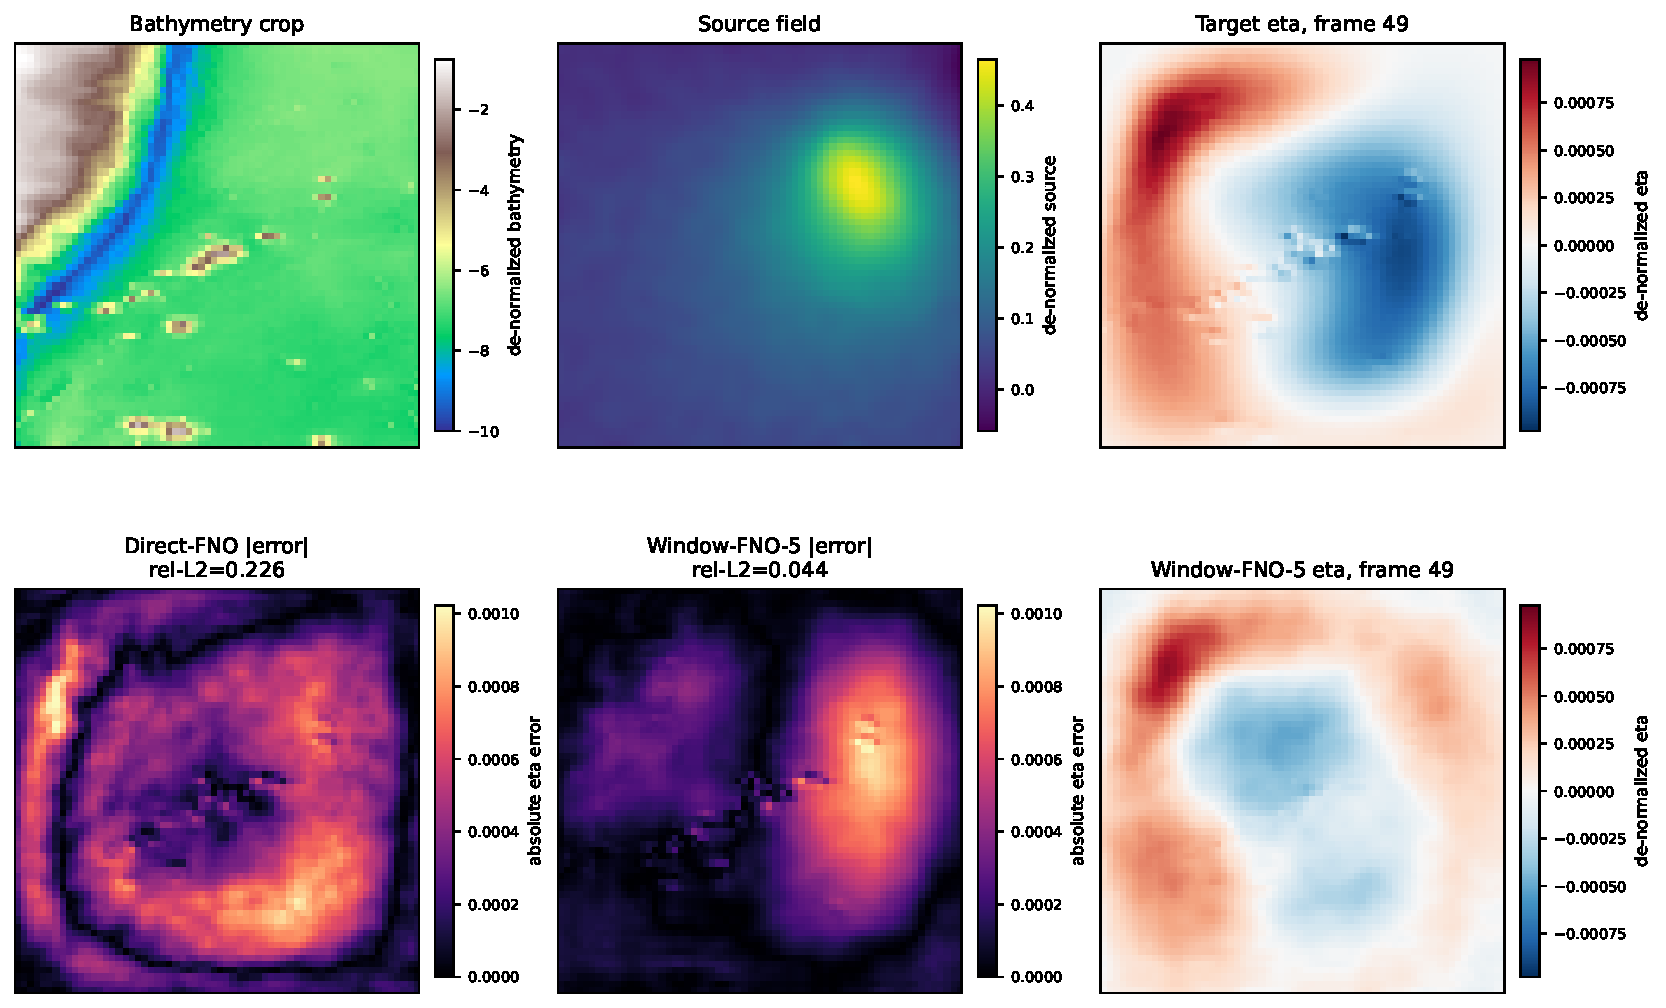
\includegraphics[width=0.7\linewidth]{figures/real_bathymetry_offshore.pdf}
\caption{Illustrative synthetic-to-real offshore morphology diagnostic on one GEBCO-derived Tohoku bathymetry crop from the real-bathymetry suite, rescaled to the fully wet training range $[-10,\, -0.75]$. Top row: de-normalized bathymetry crop, synthetic Okada-like source field, and hydrostatic reference surface elevation $\eta$ at frame 49. Bottom row: absolute error of the single-pass direct FNO, absolute error of the autoregressive Window-FNO-5, and the Window-FNO-5 predicted $\eta$ at the same frame (shares the color scale of the reference panel above it). This is a morphology-transfer diagnostic under synthetic forcing, not real-event validation.}
\label{fig:real-bath}
\end{figure}

\subsection{Solver-fidelity and cross-solver diagnostics}
\label{subsec:res-solver-fidelity}

Because the training solver is not itself ground truth, Section~\ref{subsec:cross-solver} separates two quantities: the raw physical gap between two numerical references on shared scenarios, and the surrogate error of a model trained on one reference and scored against another. Table~\ref{tab:solvergap} reports the raw solver-vs-solver gaps on all $2{,}500$ shared test scenarios, in both directions for each pair. The two shallow-water references are close: hydrostatic versus MUSCL-HR has a mean relative $L_2$ of $0.164$ (RMSE $0.00173$). Both shallow-water references are far from the weakly dispersive Boussinesq solver: hydrostatic versus Boussinesq has a mean relative $L_2$ of $0.861$ and MUSCL-HR versus Boussinesq $0.897$, an order of magnitude larger in RMSE ($\approx 0.016$--$0.017$). The reverse Boussinesq-vs-shallow-water directions give even larger relative $L_2$ ($1.60$ and $1.55$): because relative $L_2$ normalizes by the second field's norm and the Boussinesq elevation field is smaller in these scenarios, dividing by the shallow-water norm yields a smaller denominator and hence a larger ratio. The symmetric RMSE and MAE are of course direction-independent. This gap structure is expected from the physics of Section~\ref{subsec:numerical-reference-formulation}: the shallow-water references share a non-dispersive long-wave model, while the Boussinesq reference adds a weakly dispersive correction, so the cross-family gap dwarfs the within-family gap.

\begin{table}[!htbp]
\centering
\caption{Raw solver-vs-solver gaps on shared test scenarios ($N = 2500$, field $\eta$ trajectory). RMSE and MAE are physical; relative $L_2$ is a per-sample mean. The relative $L_2$ is asymmetric because it normalizes by the second solver's field norm; RMSE and MAE are symmetric.}
\label{tab:solvergap}
\begin{tabular}{llccc}
    \toprule
    Solver pair ($A$ & vs $B$) & MAE & RMSE & rel-$L_2$ \\
    \midrule
    Hydrostatic & MUSCL-HR    & $0.00084$ & $0.00173$ & $0.164$ \\
    MUSCL-HR    & Hydrostatic & $0.00084$ & $0.00173$ & $0.177$ \\
    Hydrostatic & Boussinesq  & $0.00651$ & $0.01632$ & $0.861$ \\
    Boussinesq  & Hydrostatic & $0.00651$ & $0.01632$ & $1.603$ \\
    MUSCL-HR    & Boussinesq  & $0.00692$ & $0.01690$ & $0.897$ \\
    Boussinesq  & MUSCL-HR    & $0.00692$ & $0.01690$ & $1.548$ \\
    \bottomrule
\end{tabular}
\end{table}

\paragraph{Emulator-superiority ratios.}
Table~\ref{tab:superiority} reports the emulator-superiority ratio of Section~\ref{subsec:cross-solver},
\[
    \rho(A \rightarrow B) =
    \frac{\mathrm{RMSE}(f_\theta ^ A,\, \mathrm{ref}\, B)}
         {\mathrm{RMSE}(\mathrm{ref}\, A,\, \mathrm{ref}\, B)} .
\]
The numerator is the physical RMSE of a surrogate trained on reference $A$ and scored against the targets of a \emph{different} reference $B$; the denominator is the raw $A$-vs-$B$ solver gap. Because all three references are generated on the same scenarios with identical input channels (Section~\ref{subsec:res-dataset}), a surrogate can be evaluated against another reference's targets without distribution shift in its inputs. A value $\rho<1$ would mean the surrogate is closer to $B$ than $A$'s own solver is.

Across all four cross-reference pairs the ratio exceeds one. Within the shallow-water family the hydrostatic-trained FNO scored against MUSCL-HR gives $\rho = 1.98$ and the MUSCL-HR-trained FNO against hydrostatic gives $\rho = 1.76$: the two shallow-water solvers already agree closely (Table~\ref{tab:solvergap}, gap $0.00173$), so the surrogate's own emulation error is larger than the small physical gap it would have to beat. For the cross-family pairs the Boussinesq-trained FNO scored against the hydrostatic and MUSCL-HR targets gives $\rho=1.33$ in both cases: although the raw cross-family solver gap is an order of magnitude larger ($\approx 0.016$), the Boussinesq surrogate's error \emph{on the shallow-water targets} ($\approx 0.022$) is larger still, because those targets are governed by physics it was not trained on. The consistent reading is that the emulator is not ``superior'' to the numerical reference in any of these pairs: a surrogate reproduces the solver it was trained on far better than it reproduces a different solver, and the cross-solver physical gap is not something the present surrogate closes. We regard this as the honest negative outcome of the diagnostic rather than a shortfall of the method.

\begin{table}[!htbp]
\centering
\caption{Emulator-superiority ratios from Section~\ref{subsec:cross-solver}. RMSE$_f$ is the cross-reference surrogate error and RMSE$_{AB}$ is the raw solver-gap denominator from Table~\ref{tab:solvergap}. Values $\rho<1$ would indicate surrogate superiority; all rows give $\rho>1$.}
\label{tab:superiority}
\begin{tabular}{llccc}
    \toprule
    Surrogate (trained on $A$) & vs ref $B$ & RMSE$_{f}$ & RMSE$_{AB}$ & $\rho$ \\
    \midrule
    FNO (Hydrostatic) & MUSCL-HR    & $0.00343$ & $0.00173$ & $1.98$ \\
    FNO (MUSCL-HR)    & Hydrostatic & $0.00305$ & $0.00173$ & $1.76$ \\
    FNO (Boussinesq)  & Hydrostatic & $0.02174$ & $0.01632$ & $1.33$ \\
    FNO (Boussinesq)  & MUSCL-HR    & $0.02241$ & $0.01690$ & $1.33$ \\
    \bottomrule
\end{tabular}
\end{table}

\paragraph{Normalization check.}
The cross-reference diagnostic checks both the target denormalization signature and the input-channel normalization statistics between the prediction dataset and the reference dataset. For all four pairs the input-channel signature check passes: the bathymetry and source channels share identical normalization statistics across the prediction and reference datasets (the \texttt{initial\_depth} channel is unscaled on both sides), so the surrogate sees inputs on the same scale it was trained on. The target denormalization is applied separately to prediction and reference using each dataset's own stored statistics, so the physical-unit numerator and denominator are each well defined in their native scale. The ratios are therefore reported as direct physical-unit comparisons, and the qualitative conclusion ($\rho>1$ throughout) is unaffected.

\subsection{Windowed autoregressive forecaster}
\label{subsec:res-window}

To target the per-frame drift of the single-pass models (Table~\ref{tab:perframe}), we train windowed FNO and FFNO variants on the hydrostatic reference that forecast the trajectory autoregressively in blocks of $K = 5$ frames: from an input stack $[\,\text{bathymetry},\, \text{source},\, \eta_t,\, \eta_{t - 1}\,]$ each model predicts the next five frames, then re-conditions on its own last two predicted frames and advances, covering the $50$-frame horizon in ten chunks. This trades one long-horizon prediction for several short-horizon ones at the cost of an autoregressive feedback loop.

Table~\ref{tab:window} compares the windowed models against their direct single-pass counterparts on the hydrostatic test split. Window-FNO-5 reaches a full-trajectory relative $L_2$ of $0.077$, against $0.235$ for the single-pass FNO. Window-FFNO-5 is lower again at $0.052$ (physical rel-$L_2 = 0.0513$), compared with $0.168$ for the direct FFNO. The same drift pattern remains: the windowed FFNO starts at $0.030$ and rises to $0.169$ by the final predicted frame, so it reduces but does not eliminate temporal accumulation.

\begin{table}[H]
\centering
\caption{Windowed versus direct hydrostatic models on the test split ($N = 2500$). Parameter counts are in millions. Full-traj is the global relative $L_2$; per-frame columns are relative $L_2$ at the first, mid-horizon, and final frame. Direct models predict all $50$ frames from static inputs. Windowed models are seeded with the true first frame and predict frames $1$--$49$, so the tasks are not like-for-like. Inference time is per sample on GPU.}
\label{tab:window}
\small
\begin{tabular}{lcccccc}
    \toprule
    Model & Params (M) & full-traj & frame $1$ & mid & final & infer (ms) \\
    \midrule
    Direct FNO       & $5.443$ & $0.235$ & $0.214$ & $0.325$ & $0.309$ & $0.90$ \\
    Direct FFNO      & $0.411$ & $0.168$ & $0.135$ & $0.264$ & $0.273$ & $1.66$ \\
    Window-FNO-5     & $5.439$ & $0.077$ & $0.051$ & $0.130$ & $0.172$ & $11.1$ \\
    Window-FFNO-5    & $0.407$ & $\mathbf{0.052}$ & $\mathbf{0.030}$ & $\mathbf{0.105}$ & $\mathbf{0.169}$ & $21.6$ \\
    \bottomrule
\end{tabular}
\end{table}

Two caveats are essential for a fair reading. First, the comparison is not strictly like-for-like: the windowed rollout is \emph{seeded with the true first frame} $\eta_0$ and predicts frames $1$--$49$, whereas the direct models predict all $50$ frames from the static inputs alone with no seed. Part of the windowed models' advantage at early frames therefore reflects the easier, partially observed task; the late-frame improvement is more informative but still not a clean direct-task comparison. Second, the windowed models are slower because they run ten sequential forward passes: Window-FNO-5 costs $11.1$~ms and Window-FFNO-5 costs $21.6$~ms per sample. Window-FFNO-5 is much smaller than Window-FNO-5 ($0.407$M vs $5.439$M parameters), but it is slower in this implementation, so parameter count should not be read as measured throughput. Even so, they remain orders of magnitude faster than the CPU hydrostatic reference. We also do not compute the emulator-superiority ratio for the windowed models, because their seeded numerator would be a different task from the single-pass surrogate used in Section~\ref{subsec:res-solver-fidelity}.

On the 10-crop real-bathymetry morphology suite of Section~\ref{subsec:res-real}, the same seeded pattern holds: Window-FNO-5 reaches rel-$L_2 = 0.053$ and Window-FFNO-5 reaches $0.039$, compared with $0.275$ and $0.183$ for their direct counterparts. In the appendix coastline ablation, the fully wet coastline remains easy for the windowed models, while the wet-dry version fails, so we do not use the stress result to strengthen the main transfer claim. We additionally score Window-FNO-5 on the same distribution-shift and native-resolution suites used for the single-pass FNO, with the same first-frame-seeded caveat applied throughout. The native-resolution picture is different and worth stating plainly: Window-FNO-5 is trained only at $64 \times 64$, so evaluating the same checkpoint at other native grids is a zero-shot resolution transfer. At its training resolution it scores $0.076$ (in line with the main test split), but it fails when transferred zero-shot to $32 \times 32$ ($1.101$) and $128 \times 128$ ($0.828$), mirroring the single-pass zero-shot transfer collapse in Table~\ref{tab:crossres-native-transfer}. We therefore report the windowed cross-resolution result only as a same-resolution number plus an explicit zero-shot-transfer failure, not as a native-resolution training claim. Full per-suite numbers are tabulated in the appendix (Table~\ref{tab:app-window-suites}).

\subsection{Uncertainty}
\label{subsec:res-uncertainty}
We quantify predictive uncertainty with a deep ensemble of $M = 7$ hydrostatic FNOs that differ only in random seed (seeds $11$, $22$, $33$, $44$, $55$, $66$, $77$), following the protocol of Section~\ref{subsec:uncertainty}. Table~\ref{tab:uncertainty} reports two complementary diagnostics: the empirical coverage of central Gaussian prediction intervals at four nominal levels, and the Pearson correlation between the per-element predictive standard deviation and the absolute error, on the in-distribution test split and on the three distribution-shift suites.

\begin{table}[H]
\centering
\caption{Ensemble uncertainty diagnostics for the hydrostatic FNO ($M = 7$). Coverage columns are the empirical fraction of test elements inside the nominal central interval (ideal values $0.50$/$0.80$/$0.90$/$0.95$); err--unc.\ is the Pearson correlation between predictive standard deviation and absolute error. The in-distribution row is the full $N = 2500$ test split; the remaining rows are the distribution-shift suites of Section~\ref{subsec:res-ood}.}
\label{tab:uncertainty}
\begin{tabular}{lccccc}
    \toprule
    Suite & cov$_{50}$ & cov$_{80}$ & cov$_{90}$ & cov$_{95}$ & err--unc.\ \\
    \midrule
    In-distribution             & $0.463$ & $0.700$ & $0.782$ & $0.832$ & $0.646$ \\
    \texttt{multi-gauss} subset & $0.398$ & $0.630$ & $0.721$ & $0.780$ & $0.658$ \\
    \texttt{trench} subset      & $0.488$ & $0.725$ & $0.804$ & $0.851$ & $0.648$ \\
    Extreme high strength       & $0.376$ & $0.589$ & $0.673$ & $0.728$ & $0.700$ \\
    \bottomrule
\end{tabular}
\end{table}

Two findings stand out. First, the ensemble is \emph{overconfident}: empirical coverage remains below the nominal level at every interval, with the nominal $95\%$ interval capturing $83\%$ of in-distribution targets and $73$--$85\%$ under shift. Thus the Gaussian intervals built from ensemble variance are still too narrow and should not be read as calibrated probabilities. Second, and more positively, the error--uncertainty correlation is stable and moderately strong across all settings ($0.65$--$0.70$), and is highest on the extreme high-strength tail ($0.700$). So even though the absolute scale of the uncertainty is miscalibrated, its \emph{spatial structure} tracks where the model is actually wrong, which is the property that matters for flagging untrustworthy regions of a prediction.

The behavior under shift is mixed and worth stating plainly. Coverage does not improve uniformly under distribution shift, and on the high-strength tail the normalized Gaussian negative log-likelihood is worse than in distribution ($-0.22$ versus $-1.91$), meaning the variance still fails to grow enough to match the larger errors in the most extreme regime. The \texttt{trench} bathymetry suite is the one case where coverage edges above the in-distribution level, but not enough to reach the nominal targets. We therefore treat these as reliability diagnostics rather than calibrated risk estimates: the ensemble produces a useful relative ranking of where error concentrates, but its intervals would need either more members or an explicit recalibration step before being read as probabilities. We leave larger ensembles and post-hoc calibration to future work.

\subsection{Boussinesq comparison reference}
\label{subsec:res-boussinesq}
The same-solver Boussinesq result is included in Table~\ref{tab:accuracy}: the FNO trained against the weakly dispersive reference reaches a dimensionless relative $L_2$ of $0.210$, the lowest of the three references, though as noted in Section~\ref{subsec:res-accuracy} this ordering reflects the larger Boussinesq normalization scale and reverses in physical units. The pairwise raw solver-vs-solver gaps that place this number in context, and the cross-reference emulator-superiority ratios, are reported in Section~\ref{subsec:res-solver-fidelity}.
